\documentclass{beamer}
\renewcommand\thesection{\arabic{section}}
\newcommand{\myfont}{\rmfamily\normalsize\upshape\mdseries}
\newcommand{\degree}{^\circ}
\title{\sffamily Review III(Slides 119 - 167)}
\subtitle{\textbf{Sequence \& Convergence}\\ }
\institute[UM-SJTU JI]{University of Michigan-Shanghai Jiao Tong University Joint Institute}
\author{Kulu}
\usepackage{graphicx}
\usepackage{picinpar}
\usepackage{indentfirst}
\usepackage{chemformula}
\usepackage{geometry}
\usepackage{subfigure}
\usepackage{appendix}
\usepackage{amsfonts,amsmath,amssymb}
\usepackage{enumerate}
\usepackage{float}
\usepackage{geometry}
\usepackage{latexsym}
\usepackage{listings}
\usepackage{multicol,multirow,multido}
\usepackage{tabularx}
\usepackage{ulem}
\usepackage{tikz}
\usepackage{xcolor}
\usepackage{cite}
\usepackage{setspace}
\usepackage{hyperref}
\usepackage{textpos}
\usepackage{booktabs}

\usetheme[dove]{Boadilla}
\usecolortheme{dolphin}
\useoutertheme{miniframes}
\begin{document}
\usebackgroundtemplate{\tikz\node[opacity=0.1]{
        \centerline{
\includegraphics[
                height=\paperheight]{kulu.jpg}}
    };}
\begin{titlepage}
    \begin{center}
        VV186 - Honors Mathmatics II
    \end{center}
\end{titlepage}
\myfont

\section{Midterm}
\begin{frame}
    \frametitle{Midterm is Coming}
    \begin{figure}[htbp]
        \centering
        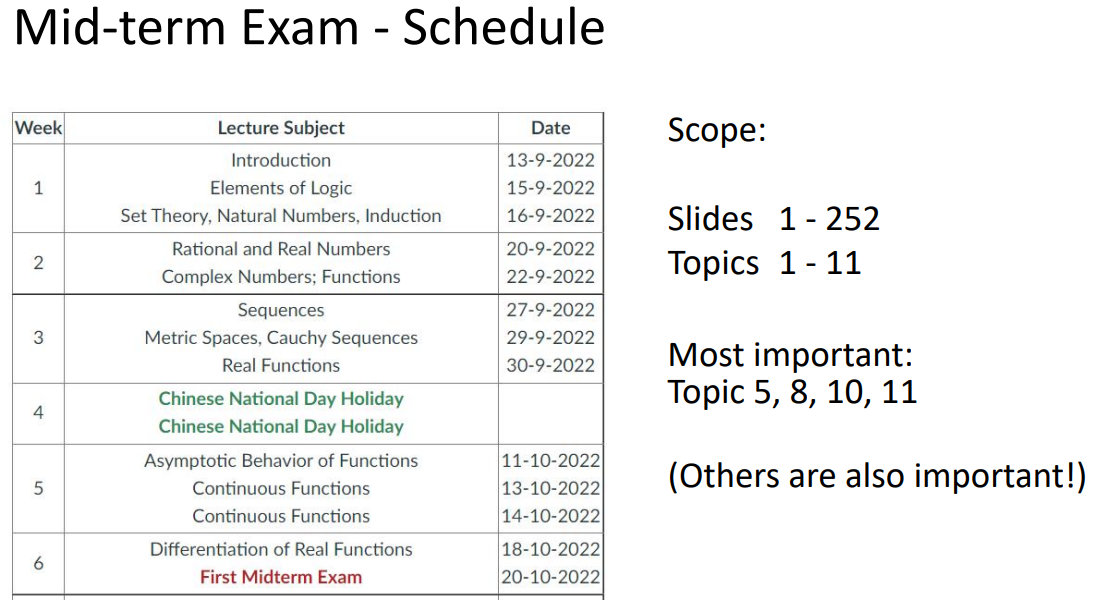
\includegraphics[width=12cm]{syllabus.png}
    \end{figure}
\end{frame}

\begin{frame}
    \frametitle{Midterm Preparation}
    \begin{figure}[htbp]
        \centering
        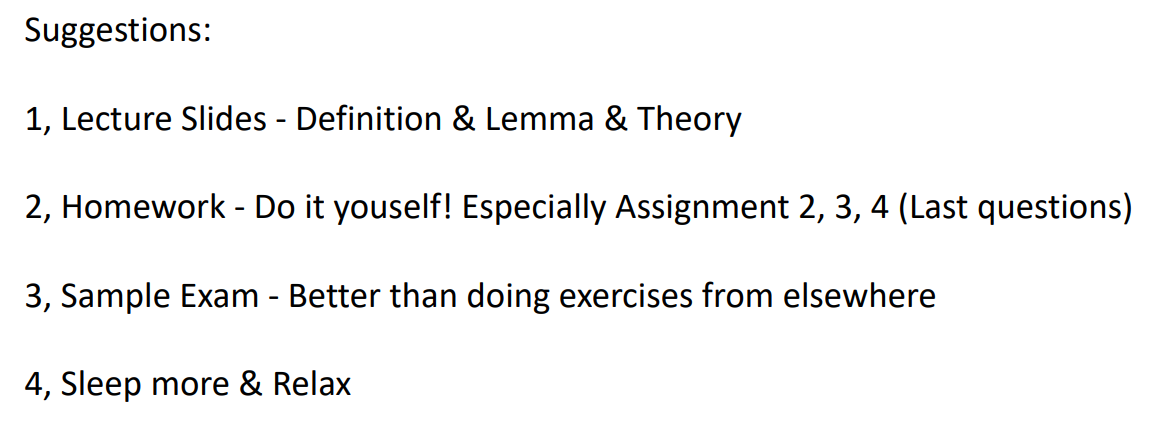
\includegraphics[width=12cm]{preparation.png}
    \end{figure}
    \textcolor{red}{Kulu's Personal Tips:}
    \begin{itemize}
        \item Understanding instead of reciting ! Explain concepts and theories in your own intuitive words.
        \item Visualize is most important. For set, for function, for sequence.
    \end{itemize}
\end{frame}

\section{Set}
\begin{frame}
    \frametitle{$\overline{lim}$ and $\underline{lim}$ for set}
    First, let's recall the definition.
    \begin{figure}[htbp]
        \centering
        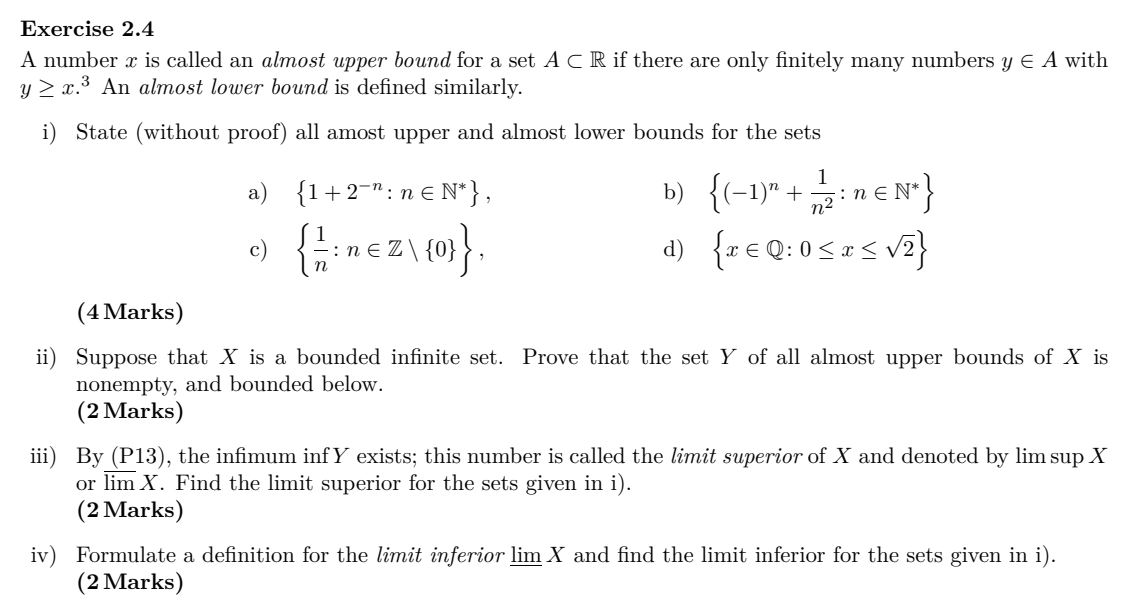
\includegraphics[width=12cm]{definition.png}
    \end{figure}
\end{frame}

\begin{frame}
    \frametitle{$\overline{lim}$ and $\underline{lim}$ properties}
    Prove them “in a second”. Be familiar enough with every concept and conclusion in your assignment !

    Warning: A finite set doesn't necessarily have a maximum/minimum ! It can be empty !

    \begin{figure}[htbp]
        \centering
        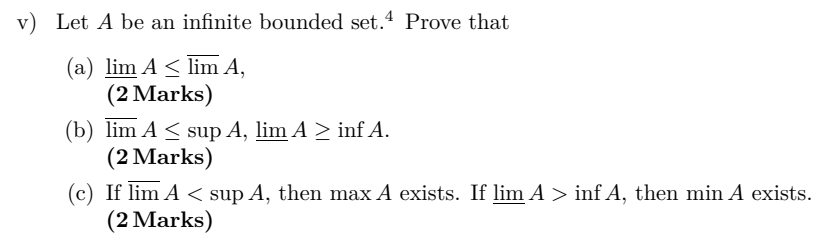
\includegraphics[width=12cm]{properties.png}
    \end{figure}
\end{frame}

\begin{frame}
    \frametitle{Proof for $\overline{lim}$ and $\underline{lim}$ properties}
\end{frame}

\begin{frame}
    \frametitle{Exercise (Left in RC2)}
    \begin{figure}[htbp]
        \centering
        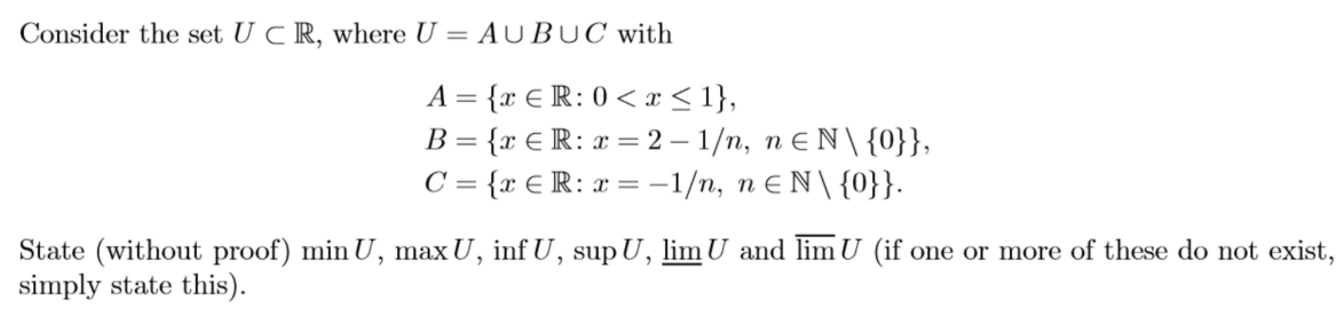
\includegraphics[width=12cm]{extra2.png}
    \end{figure}
\end{frame}

\begin{frame}
    \frametitle{Exercise Answer (Left in RC2)}
    \begin{figure}[htbp]
        \centering
        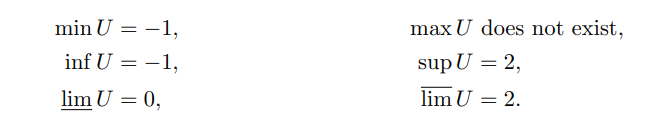
\includegraphics[width=12cm]{answer.png}
    \end{figure}
\end{frame}

\begin{frame}
    \frametitle{Exercise (Left in RC2)}
    Question: When does inf/sup exist? When does $\overline{lim}$ and $\underline{lim}$ exist?
    \begin{figure}[htbp]
        \centering
        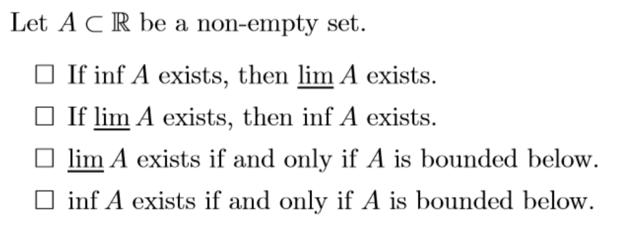
\includegraphics[width=12cm]{extra.png}
    \end{figure}
\end{frame}

\section{Sequence}
\begin{frame}
    \frametitle{Sequence}
    Last year, a lot of students asked Prof. and TAs:
    \begin{itemize}
        \item Why is a sequence always have infinite items?
        \item What if a sequence only have finite items?
        \item ...
    \end{itemize}

    \textcolor{red}{!!!}
    When we say “sequence” we usually assume that it is infinite.\\
    If it is finite, i.e., it contains only finite items
    , we usually say it is a “n-tuple”.
    Similarly, a subsequence of a sequence is infinite.

\end{frame}
\begin{frame}
    \frametitle{Convergence \& Divergence}
    \begin{block}{Quick check:}
        \hspace{1em}
        \begin{itemize}
            \item A sequence is either convergent or divergent to (minus) infinity.
            \item A sequence is either convergent or divergent.
            \item If a sequence diverges, then it will go to (minus) infinity.
        \end{itemize}
    \end{block}
\end{frame}

\begin{frame}
    \frametitle{Relationship between limit and accumulation set}
    First, recall the definition:
    \begin{itemize}
        \item Limit:
              \begin{itemize}
                  \item How to impretate it ?
                  \item Relationship with boundness ?
                  \item How many limits a sequence can have ?
              \end{itemize}
        \item Accumulation Point:
              \begin{itemize}
                  \item How to impretate it ?
                  \item How many accumulation points can a sequence have ?
                  \item limit of the subsequence ?
                  \item Existence ?
                  \item Relationship with boundness ?
                  \item Difference between accumulation points for set and sequence ?
                        Accumulation point of ran$(a_{n})$ must be accumulation point for $(a_{n})$ ?
                        Vice versa ?
              \end{itemize}
    \end{itemize}
\end{frame}

\begin{frame}
    \frametitle{Limit}
    Some  results for limit.\\
    \begin{center}
        Suppose $(a_n)\rightarrow a \in \mathbb{R}$ and $(b_n)\rightarrow b \in \mathbb{R}$
    \end{center}
    \begin{enumerate}
        \item $\lim (a_n+b_n)=a+b$
        \item $\lim (a_n\cdot b_n) =a\cdot b$
        \item $\lim \frac{a_n}{b_n}=\frac{a}{b}, b\neq 0$
    \end{enumerate}
    We will prove property 3 later.

    Useful conclusion: if ($a_{n}$) converges to a > 0, $\forall x \in (0,a)$, there exists N>0, such that $\forall n > N$, $a_{n}>x>0$. \textcolor{red}{Visualize it to understand}
    \begin{block}{Notice:}
        \hspace{1em}
        $\lim (a_n+b_n)=\lim a_n + \lim b_n$?

        \quad $\underset{n\rightarrow \infty}{lim(\left|a_{n+1}-a_{n}\right|)}=0$, then ($a_{n}$) converges?
    \end{block}
\end{frame}
\begin{frame}
    \frametitle{Limit}
    \begin{center}
        $\lim \frac{a_n}{b_n}=\frac{a}{b}, b\neq 0$
    \end{center}
    Look at the definition and set your goal!
    \begin{block}{Goal:}
        \hspace{10em}
        $$\underset{\varepsilon>0}{\forall}~ \underset{N>0}{\exists} ~\underset{n>N}{\forall}~ |\frac{a_n}{b_n}-\frac{a}{b}|<\varepsilon$$
    \end{block}
    \textbf{Another approach:}\\
    \hspace{1em} Using the second result and try to prove $\lim \frac{1}{b_n}=\frac{1}{b}$
\end{frame}
\begin{frame}
    \frametitle{Proof}
\end{frame}

\begin{frame}
    \frametitle{Exercises : Important limits}
    \begin{figure}[htbp]
        \centering
        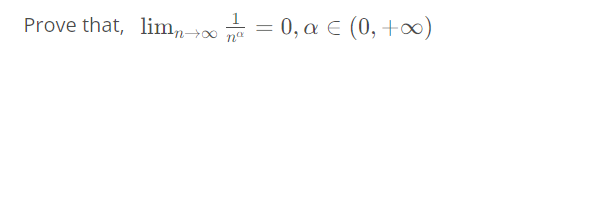
\includegraphics[width=12cm]{limit1.png}
    \end{figure}
\end{frame}

\begin{frame}
    \frametitle{Exercises : Important limits}
    \begin{figure}[htbp]
        \centering
        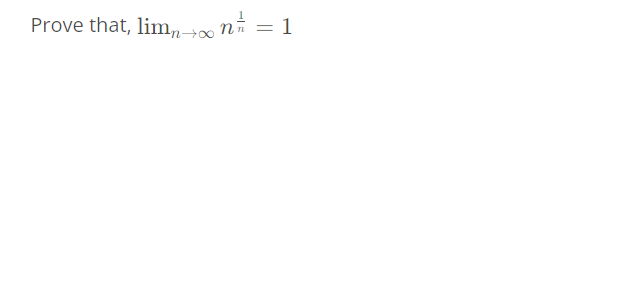
\includegraphics[width=12cm]{limit2.png}
    \end{figure}
\end{frame}

\begin{frame}
    \frametitle{Exercises : Important limits}
    \begin{figure}[htbp]
        \centering
        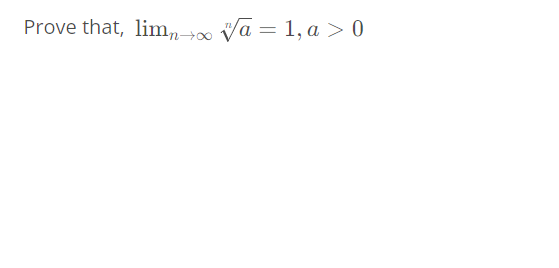
\includegraphics[width=12cm]{limit3.png}
    \end{figure}
\end{frame}

\begin{frame}
    \frametitle{Exercises}
    Let ($a_n$) be a sequence that $a_n=\frac{1}{\sqrt{n^2+1}}+\cdots+\frac{1}{\sqrt{n^2+n}}$.
    Calculate the limit of ($a_n$).
\end{frame}

\begin{frame}
    \frametitle{Exercises}
    A sequence is defined as
    \begin{equation*}
        (S_n)_{n\in\mathbb{N}}, S_1=\sqrt{2}, S_2=\sqrt{2+\sqrt{2}}, S_3=\sqrt{2+\sqrt{2+\sqrt{2}}},...
    \end{equation*}
    Please prove that it is convergent and calculate the limit of $(S_n)$ as $n\rightarrow \infty$.
\end{frame}

\begin{frame}
    \frametitle{Exercises \textcolor{red}{(Important)}}
    \begin{figure}[htbp]
        \centering
        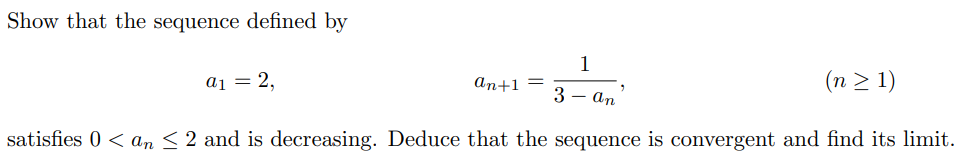
\includegraphics[width=12cm]{sequenceExercise.png}
    \end{figure}
\end{frame}

\begin{frame}
    \frametitle{Exercises}
    Let $(a_n),(b_n)$ be two real sequences. Furthermore, assume that $a_n<b_n$
    for all $n$, $[a_{n+1}, b_{n+1}]\subseteq [a_n,b_n]$, $\lim (a_n-b_n)=0$. Prove that there
    is an unique $m\in [a_n,b_n]$ for all $n$, such that
    \begin{equation*}
        \lim a_n=\lim b_n=m
    \end{equation*}
\end{frame}
\begin{frame}
    \frametitle{Exercises}
    Let ($a_n$) be a real sequence that converges to $a \in \mathbb{R}$.
    Prove that the sequence ($\frac{\sum_{i=1}^n a_i}{n}$) is convergent.
    Furthermore $\underset{n\rightarrow \infty}{\lim} (\frac{\sum_{i=1}^n a_i}{n})=a $.
\end{frame}

\begin{frame}
    \frametitle{Exercises}
    Let ($a_n$) be a real sequence that converges to $a \in \mathbb{R}$.
    Let ($b_n$) be a real sequence that converges to $b \in \mathbb{R}$.
    Prove that the sequence ($\frac{\sum_{i=1}^n a_{i}b_{n-i+1}}{n}$) is convergent.
    Furthermore $\underset{n\rightarrow \infty}{\lim} (\frac{\sum_{i=1}^n a_{i}b_{n-i+1}}{n})=ab$.
\end{frame}


\begin{frame}
    \frametitle{$\overline{lim}$ and $\underline{lim}$ for sequence }
    How to interpret $\overline{lim}$ and $\underline{lim}$ of a sequence ?
    \begin{itemize}
        \item Way 1: Let $\alpha_{n}=\mathop{inf}\limits_{k\geq n}a_{k}$, $\overline{lim} a_{n}$=$\mathop{lim}\limits_{n\rightarrow \infty}\alpha_{n}$
        \item Way 2: Largest and smallest accumulation point.
    \end{itemize}
    Properties:
    \begin{itemize}
        \item Important property:
              \vspace*{1em}
              $\forall x > \overline{lim} a_{n}$, $\exists N\in \mathbb{N}$, such that $\forall n \geq N, a_{n} < x$.

        \item Property in Assignment:

              \vspace*{1em}
              $\overline{lim}a_{n}$ $\geq$ $\underline{lim}a_{n}$


              \vspace*{1em}
              $\overline{lim} a_{n}$ = $\overline{lim} ran(a_{n})$
    \end{itemize}
\end{frame}

\begin{frame}
    \frametitle{Exercise}
    \begin{figure}[htbp]
        \centering
        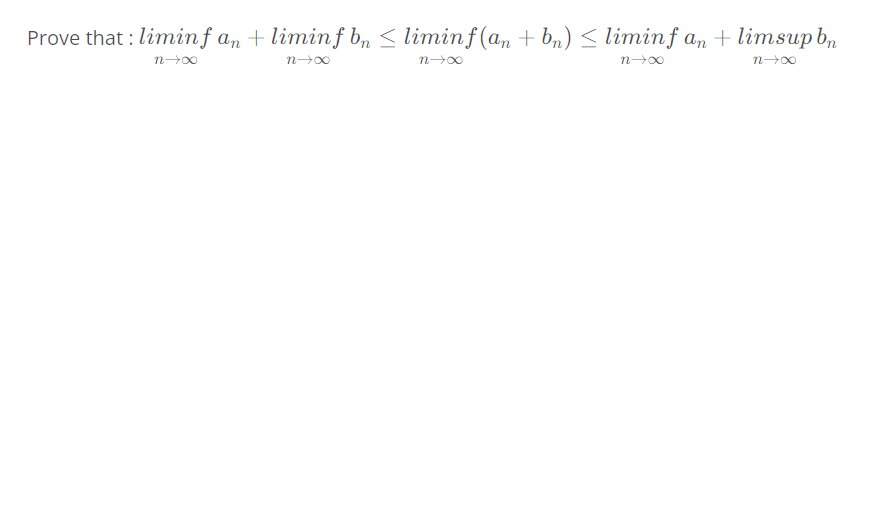
\includegraphics[width=12cm]{infsup.png}
    \end{figure}
\end{frame}


\begin{frame}
    \frametitle{Important Results \& Theorem}
    \begin{itemize}
        \item A convergent sequence is bounded. (Slides 128)
        \item A convergent sequence has precisely one limit. (Slides 130)
        \item (\textbf{Squeeze Theorem}) \\Let $(a_n),(b_n)$ and $(c_n)$ be real sequences with $a_n<c_n<b_n$
              for sufficiently large $n\in\mathbb{N}$. Suppose that $\lim\ a_n=\lim\ b_n=:a$. Then
              $(c_n)$ converges and $\lim\ c_n=a$. (Slide 133)\\
              \itshape{Comment:} It is extremely useful for examining the convergence of a sequence that is bounded.
              \myfont
        \item Let $(a_n)$ be a convergent sequence with limit $a$. Then any subsequence of $(a_n)$
              is convergent with the same limit. (Slide 145)
        \item Every real sequence has a monotonic subsequence. (Slide 146)
    \end{itemize}
    \vspace{1em}
    \textcolor{red}{Refer to slides, check the proofs on the weekend!}
\end{frame}
\begin{frame}
    \frametitle{Important Results \& Theorem}
    \begin{itemize}
        \item If a sequence has an accumulation point $x$, then there is a subsequence that converge to this point $x$. (Slides 149)
        \item (\textbf{Bolzano--Weierstraß})\\ Every bounded real sequence has an accumulation point. \\(Slide 150)\\
              \itshape{Comment.} There are at least two proofs, which we will discuss later.
        \item \myfont Every monotonic and bounded (real) sequence is convergent. (Slide 141)\\
              \itshape{Comment.} This result holds for sequence in any space with an ordering (otherwise it's
              strange to even define ''monotonic").
    \end{itemize}
    \vspace{1em}
    \textcolor{red}{Refer to slides, check the proofs on the weekend!}
\end{frame}
\begin{frame}
    \frametitle{Bolzano--Weierstraß}
    \textbf{Bolzano--Weierstraß} Every bounded real sequence has an accumulation point.
    \begin{enumerate}
        \item Proof--1: On Horst's Slides.
        \item Proof--2:
              Since$(a_n)$ is bounded, assume $-M\leq a_n\leq M$ for all n. Divide the interval $[-M,M]$ into 2 sections:$[-M,0],[0,M]$.\\
              One of the interval, denoted by $I^{(1)}$, must contain infinitely many ''$a_n$"s(otherwise $(a_n)$is finite). Choose an $a_{(n,1)}$
              in $I^{(1)}$. We bisect $I^{(1)}$ into two intervals, one of which, denoted by $I^{(2)}$ must contain
              infinitely many ''$a_n$ "s. Choose an $a_{(n,2)}$ in $I^{(2)}$ that is different from $a_{(n,1)}$ . By
              repeatedly doing this procedure, we find a subsequence $(a_{n,k})_{k\in\mathbb{N}}$ that converges.
    \end{enumerate}
\end{frame}


\section{Metric Space}
\begin{frame}
    \frametitle{Metric Space}
    \begin{itemize}
        \item What is the definition of a metric?
        \item Why we want to introduce the idea of Metric Space?
        \item What new results can we explore from this new idea?
    \end{itemize}
    We want to generalize the idea of \textcolor{red}{convergence}, or close to some point.
    The most important thing is to define
    the \textbf{Length Function}. Metric is just a \textcolor{blue}{nice} way of describing the
    \textcolor{blue}{distance}.\\

    \vspace{1em}
    What properties a usual length function should have?
    \begin{enumerate}
        \item Always positive.(distance)
        \item Symmetric.(distance)
        \item Followed \emph{Triangle Inequality}.(nice)
    \end{enumerate}
    \vspace{0.5em}
    The remaining task is just
    transform these into mathematical language\dots
\end{frame}
\begin{frame}
    \frametitle{Metric Space}
    A two variables functions
    $\rho(\cdot,\cdot):M\times M \rightarrow \mathbb{R}$
    is called a metric if it satisfies:
    \begin{enumerate}
        \item $\forall x,y\in M,\ \rho (x,y) \geq 0$ and $\rho (x,y)=0$ if and only if $x=y$.
        \item  $\forall x,y\in M,\ \rho (x,y)=\rho (y,x)$.
        \item  $\forall x,y,z\in M,\ \rho (x,z)\leq \rho (x,y)+\rho (y,z)$.
    \end{enumerate}

    Examples:
    \begin{itemize}
        \item $M=\mathbb{R}^n$, the usual metric is given by
              \begin{equation*}
                  \rho ( (x_1,x_2,\dots,x_n), (y_1,y_2,\dots,y_n)) = \sqrt{\sum^{n}_{i=k}(x_i-y_i)^2 }
              \end{equation*}
              and this is so-called \emph{Euclidean distance}.
        \item $M=\mathbb{N}, \rho(x,y)= \#\{ a:a\in [min\{x,y\},max\{x,y\}]\ \} $
        \item $M=\mathbb{R},\rho (x,y)=1 $ if $x\neq y$; $\rho (x,y)=0$ if $x=y$
    \end{itemize}
\end{frame}
\begin{frame}
    \frametitle{Generalization of Convergence}
    Then, by replacing the usual matric $\rho(x,y)=|x-y|$ and choosing our universal set $M$, we get the natural definition for
    generalize convergence in metric space $(M,\rho)$ for a sequence $(a_n):\mathbb{N}\rightarrow M$, which is given by:
    \begin{equation*}
        \lim_{n\rightarrow \infty}a_n=a\quad :\Leftrightarrow \quad \underset{\varepsilon>0}{\forall}\ \underset{N\in \mathbb{N}}{\exists}\ \underset{n>\mathbb{N}}{\forall} a_n\in B_\varepsilon(a)
    \end{equation*}
    where
    \begin{equation*}
        B_\varepsilon(a)=\{ x\in M:\rho(x,a)<\varepsilon\},\quad \varepsilon>0,\quad a\in M.
    \end{equation*}
\end{frame}

\begin{frame}
    \frametitle{Cauchy Sequences}
    A Sequence ($a_n$) in a metric space ($M$, $\rho$) is called a
    \textbf{Cauchy Sequence} if
    $$\underset{\varepsilon>0}{\forall} ~\underset{N \in \mathbb{N}}{\exists}~\underset{m,n>N}{\forall} ~\rho(a_m,a_n)<\varepsilon$$
    An intuitive description of a Cauchy sequence is that the elements are
    getting closer together.\\
    \vspace{1em}
    \textcolor{red}{Some properties:}
    \begin{enumerate}
        \item Every Cauchy sequence is bounded.
        \item Every convergent sequence is a Cauchy sequence.
        \item But not every Cauchy sequence converges.
        \item If all Cauchy sequences in a metric space converges,
              then the space is called \textbf{complete}.
    \end{enumerate}
\end{frame}

\begin{frame}
    \frametitle{Complete and Incomplete Metric Spaces}
    A metric space is complete when all cauchy sequence in this metric space converges.
    \begin{figure}[htbp]
        \centering
        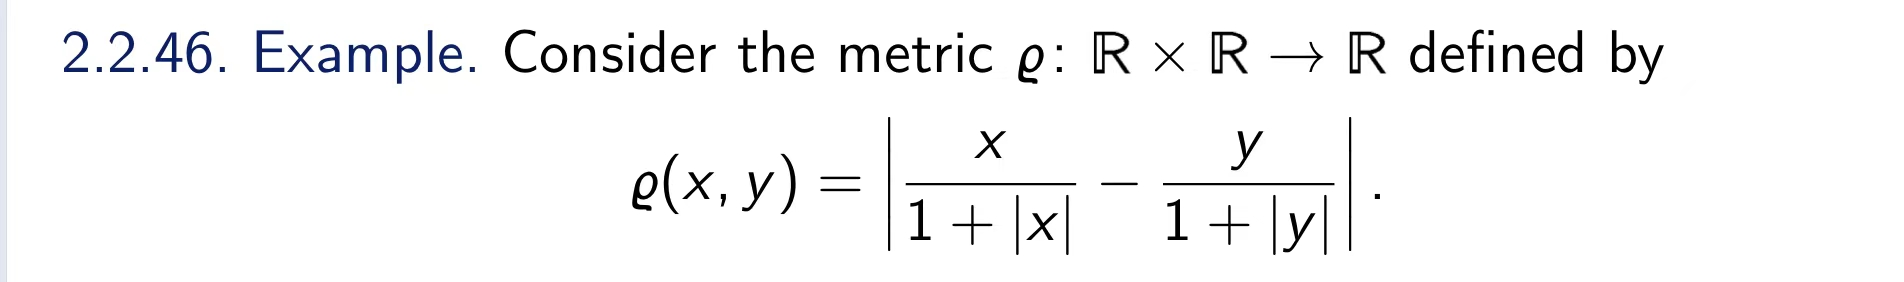
\includegraphics[width=12cm]{complete.png}
    \end{figure}
    The metric space $(\mathbb{R},\rho)$ is incomplete. (Know that the metric space can be incomplete)

    The metric space $(\mathbb{Q},\left|\cdot\right|)$ is incomplete. (Should remember)

    The metric space $(\mathbb{Q},\left|\cdot\right|)$ is complete. (Should remember)
\end{frame}




\begin{frame}
    \frametitle{For $\rho$(x,y)=$\left|x-y\right|$, ($\mathbb{C}$, $\rho$) is complete}
    In the lecture we have discussed that ($\mathbb{R}$, $\rho$) is complete.
    For every Cauchy sequence ($z_n$) in $\mathbb{C}$,
    we can write it into 2 real sequences ($x_n$) and ($y_n$)
    by writing $z_n = x_n + i \cdot  y_n$. Since
    $$(x_m-x_n)^2\leq (x_m-x_n)^2+(y_m-y_n)^2=|z_m-z_n|^2<\varepsilon$$
    $$\Rightarrow |x_m-x_n|< \varepsilon$$
    and similar for ($y_n$), both ($x_n$) and ($y_n$) are Cauchy and thus convergent.
    Since a complex sequence converges if the real and imaginary parts
    converge, ($z_n$) converges and $\mathbb{C}$ is complete.

\end{frame}



\begin{frame}
    \frametitle{Exercise \textcolor{red}{Important!} (A Former Midterm Question)}
    Prove that every Cauchy sequence has at most one accumulation point.

    \vspace{2em}
    Tips:
    \begin{itemize}
        \item You should work on an abstract metric space, using $\rho $ instead of $| \cdot |$.
        \item \textcolor{red}{Visualize to help you think !}
    \end{itemize}
\end{frame}

\begin{frame}
    \frametitle{Get familiar with Cauchy !}
    Given a sequence $(a_{n})$, And define the sequence $(b_{n})$ as:
    \begin{equation*}
        b_{n} = \sum_{i=1}^{n}\left|a_{n+1}-a_{n}\right|
    \end{equation*}
    Prove that if $(b_{n})$ is bounded, ($a_{n}$) converges.

    Tips:
    \begin{itemize}
        \item Cauchy is really useful for proving convergence !
        \item Think about how you can get the difference between two distant $a_{i}$ and $a_{j}$.
    \end{itemize}
\end{frame}

\begin{frame}
    \frametitle{Get familiar with Cauchy !}
    \begin{figure}[htbp]
        \centering
        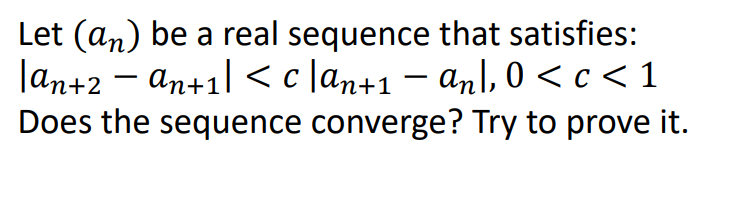
\includegraphics[width=12cm]{challenge.png}
    \end{figure}

    Tips:
    \begin{itemize}
        \item Cauchy is really useful for proving convergence !
        \item Think about how you can get the difference between two distant $a_{i}$ and $a_{j}$.
    \end{itemize}
\end{frame}


\begin{frame}
    \frametitle{Reference}
    \begin{itemize}
        \item VV186 Lecture Slides Horst Hohberger
        \item 2021 Vv186 TA-Niyinchen
        \item 2022 Vv186 TA-Dingzizhao
        \item 2022 Vv186 TA-Sunmeng
        \item 2022 Vv186 TA-Matianyi
    \end{itemize}

\end{frame}
\end{document}